In this section the system described will be modelled and validated using AlloyTools. The analysis is divided in 4 main parts:
\begin{itemize}
    \item Static Analysis;
    \item Dynamic Analysis;
    \item Assertions;
    \item Word Generation;
\end{itemize}
For this analysis the following assumptions have been considered:
\begin{itemize}
    \item The Float type (not defined) represents a decimal number;
    \item A \ac{CPO} can be modelled without being a part of the \ac{eMSP};
\end{itemize}

\subsection{Static Analysis}
Here the model is created, all the classes are represented by a \textbf{sig}. For the purpose of this analysis only the relational properties are considered, so the attributes of basic types (such as Int,float,boolean,Data etc...) are not considered.
This decision has been taken to simplify the model view and coding. Most platforms that could be used to implement the system, already support this or similar types of data.\\
As a guideline the types are written only in the declarations inside a comment; they are defined by unimplemented interfaces and their ranges are specified; this types are not considered in the rest of the document.

\begin{verbatim}
    module eMall

    //only CPMS used in the system are added
    
    //-------SIG-----
    
    
    
    sig CPO{
        cpms: set CPMS
        //name: one String
        //email: one Email
        //pIVA: one Int
        //iban: one Int
        //password: one String
    }
    
    
    sig EMSP{
        users: set DefaultUser,
        charges: set Charge,
        cpos:set CPO
    }
    
    sig CPMS{
        stations:set ChargingStation,
        maintainers:set Maintainer
    }
    
    abstract sig User{
        //name: one Str,
        //surname: one Str,
        //birthday: one Date,
        //mail: one Str,
        //password: one Str,
    } 
    sig DefaultUser extends User{
        vehicles: set Vehicle
        //paymentInfo: one String
    }
    sig Maintainer extends User{}
    
    sig Vehicle{
        //batteryLevel: one Int,
        //KWperKm: one Int,
        location: one Location
    }
    //{ 
        //inRange[batteryLevel, 0, 100]
        //inRange[KWperKm, 0, 100]}
    
    sig ChargingStation{
        position:one Location,
        //batteryKWh: one Int,
        sockets: set ChargingSocket,
        strategy: one Strategy
        //bookedCharges: one Map	
    } 
    //{  batteryPresent.isTrue implies inRange[batteryKWh, 0, 1000]}
    
    sig ChargingSocket{
        chargingType: one ChargingType,
        //available: one Bool,
        //maximumPowerAmount: one Int,
        energySource:one EnergySource
    }
    //{ inRange[maximumPowerAmount, 0, 1000]}
    
    sig Charge{
        //paid: one Bool,
        station: one ChargingStation,
        user: one DefaultUser
        //confirmationId; one String,
        //amount: one Int,
        //date: one Date
    }
    
    abstract sig Strategy{}
    one sig Manual extends Strategy{}
    one sig Automatic extends Strategy{}
    
    abstract sig ChargingType{}
    one sig SuperFast extends ChargingType{}
    one sig Fast extends ChargingType{}
    one sig Normal extends ChargingType{}
    
    abstract sig EnergySource{
        //costPerKw: one Float
    }
    //{ inRange[costPerKw, 0, 10000]}
    sig Battery extends EnergySource{
    //capacity: one Int
    }
    sig DSO extends EnergySource{}
    
    //utils types
    
    //sig Date{}
    
    //sig Str{}
    
    //simplified using int
    sig Location{  
        //latitude: one Int,   
        //longitude: one Int
    }
    //{  inRange[latitude, -90, 90] and   
    //	inRange[longitude, -180, 180]}
    
    //-------FACTS------
    
    //fact uniqueMailForUser{
        //no disjoint u1,u2: User | u1.mail = u2.mail}
    
    //fact uniqueMailForCPO{
        //no disjoint c1,c2: CPO | c1.mail = c2.mail}
    
    fact uniqueLocationForStation{
        no disjoint s1,s2: ChargingStation | s1.position = s2.position}
    
    fact uniqueCPOForCPMS{
        no disjoint c1,c2: CPO, cp:CPMS | cp in c1.cpms and cp in c2.cpms}
    
    fact uniqueCPMSForStation{
        no disjoint c1,c2: CPMS, s:ChargingStation | 
        s in c1.stations and s in c2.stations}
    
    fact socketOnlyOneStation{
        all s:ChargingSocket| s in ChargingStation.sockets
        no disjoint c1,c2: ChargingStation, s:ChargingSocket|
        (s in c1.sockets and s in c2.sockets)}
    
    fact noVehicleWithoutUser{
        all v:Vehicle|  v in DefaultUser.vehicles}
    
    fact noStationWithoutCPMS{
        all s:ChargingStation|  s in CPMS.stations}
    
    fact noUserWithoutEMSP{
        all u:DefaultUser|  u in EMSP.users}
    
    fact noChargeWithoutEMSP{
        all c:Charge|  c in EMSP.charges} 
    
    fact noChargeWithoutUserInTheEMSP{
        all c:Charge| c in EMSP.charges and c.user in EMSP.users}
    
    fact allChargeAreFromChargingStationInTheEMSP{
        all e:EMSP,s:e.charges.station | s in e.cpos.cpms.stations }
    
    fact maintainersMaintainStationOfTheSameCPO{
        all m:Maintainer, c1,c2:CPO|
        (not c1=c2 and m in c1.cpms.maintainers) implies 
        m not in c2.cpms.maintainers }
    
    fact chargingStationThatChargeHasToHaveAtLeastOneSocket{
        all c:ChargingStation | c in Charge.station implies #c.sockets>0}
        
\end{verbatim}

\subsection{Dynamic Programming}
In this part the major operations are described and run; as a convention old represents the version before the execution of the predicate, while the new is the version after the execution.\\
The picture here shown are cut to emphasize the predicate result.

\subsubsection{User books a charge}
\begin{verbatim}
    pred UserCreatesACharge(new,old:EMSP,u:DefaultUser, s:ChargingStation){
        one c:Charge  | u in new.users and
        c.user=u and c.station=s and  
        (not (new = old)) and  
        new.users=old.users and
        new.cpos=old.cpos and 
        new.charges=old.charges+c
    }
    run UserCreatesACharge for 3 but exactly 2 EMSP  
\end{verbatim}

\begin{figure}[H]
    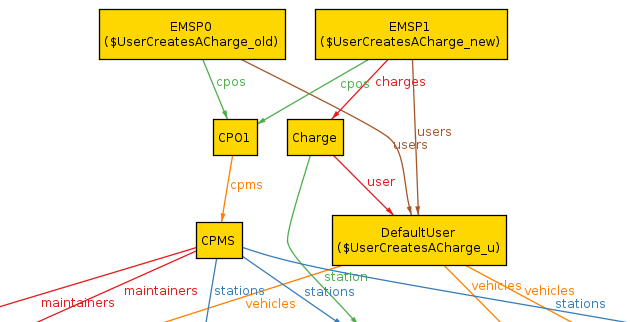
\includegraphics[keepaspectratio, width=16cm]{Alloy/UserCreateCharge.png}
    \caption{Added Charge}
\end{figure}

\subsubsection{CPO subscribe to EMSP}
\begin{verbatim}
    pred CPOSubscribeItselfToEMSP(new,old:EMSP,cpo:CPO){
        not (old = new)
        new.charges=old.charges
        new.users= old.users
        new.cpos=old.cpos+cpo
    }
    run CPOSubscribeItselfToEMSP for 3 but exactly 2 EMSP, exactly 2 CPO             
\end{verbatim}
\begin{figure}[H]
    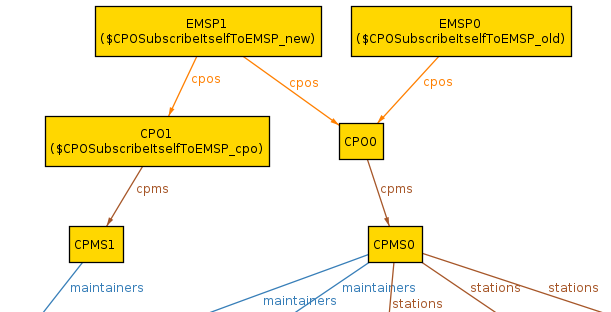
\includegraphics[keepaspectratio, width=16cm]{Alloy/CpoSubscribe.png}
    \caption{CPO subscribed}
\end{figure}

\subsubsection{CPO add CPMS}
\begin{verbatim}
    pred CPOAddCPMS(new,old:CPO,cp:CPMS){
        not (old = new)
        new.cpms=old.cpms+cp
    }
    run CPOAddCPMS for 3 but exactly 2 CPO, exactly 2 CPMS   
\end{verbatim}
\begin{figure}[H]
    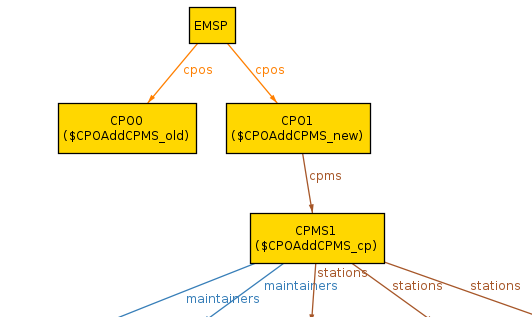
\includegraphics[keepaspectratio, width=16cm]{Alloy/CpoAddCPMS.png}
    \caption{Added CPMS}
\end{figure}

\subsubsection{CPO remove CPMS}
Only one remove is shown since they are logically identical to their corresponding adds.
\begin{verbatim}
    pred CPORemoveCPMS(new,old:CPO,cp:CPMS){
        not (old = new)
        cp in old.cpms
        new.cpms=old.cpms-cp
    }
    run CPORemoveCPMS for 3 but exactly 2 CPO, exactly 2 CPMS
\end{verbatim}
\begin{figure}[H]
    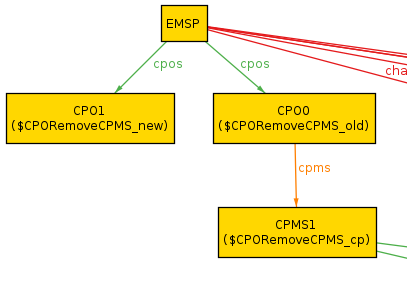
\includegraphics[keepaspectratio, width=16cm]{Alloy/remove.png}
    \caption{Removed CPMS}
\end{figure}



\subsubsection{CPO add mantainer to CPMS}
\begin{verbatim}
    pred CPOAddMaintainerToCPMS(c:CPO,new,old:CPMS,m:Maintainer){
        not (new = old)
        old in c.cpms
        new in c.cpms
        new.stations=old.stations
        new.maintainers=old.maintainers+m
    }
    run CPOAddMaintainerToCPMS for 3 but exactly 2 CPMS   
\end{verbatim}
\begin{figure}[H]
    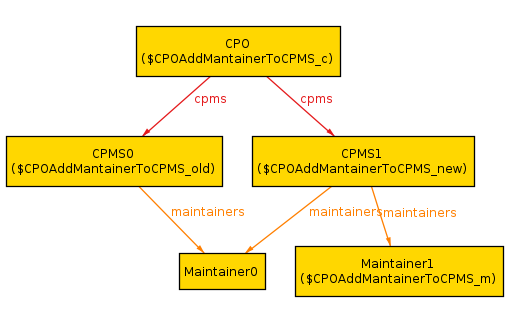
\includegraphics[keepaspectratio, width=16cm]{Alloy/CpoAddMaintainer.png}
    \caption{Added Maintainer}
\end{figure}

\subsubsection{CPO add station to CPMS}
\begin{verbatim}
    pred CPOAddStationToCPMS(c:CPO,new,old:CPMS,s:ChargingStation){
        not (new = old)
        old in c.cpms
        new in c.cpms
        new.maintainers = old.maintainers
        new.stations=old.stations+s
    }
    run CPOAddStationToCPMS for 3 but exactly 2 CPO    
\end{verbatim}
\begin{figure}[H]
    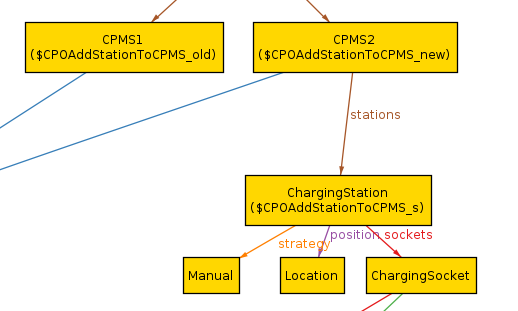
\includegraphics[keepaspectratio, width=16cm]{Alloy/CpoAddStation.png}
    \caption{Added Station}
\end{figure}

\subsubsection{CPO add socket to station}
The following code does not solve; the add pattern used here consist in creating a new instance representing the status after the execution of the predicate. As a fact a socket can exist only in one station rendering this function inconsistent; this is due a limitation of the pattern, not the model, so in this document it is considered valid.

\begin{verbatim}
    pred CPOAddSocketToStation
    (c:CPO,cp:CPMS, new,old:ChargingStation,sk:ChargingSocket)
    {
        not (new = old)
        cp in c.cpms
        new in cp.stations
        old in cp.stations
        new.position=old.position
        new.strategy=old.strategy
        new.sockets=old.sockets+sk
    }  
\end{verbatim}

\subsection{Assertions}
Here we check the validity of the model trough the Assert notation.
\begin{verbatim}
    //Asserts

    assert uniqueLocationForStationCheck{
        no disjoint s1,s2: ChargingStation | s1.position = s2.position}
    check uniqueLocationForStationCheck for 10
    
    assert uniqueCPOForCPMSCheck{
        no disjoint c1,c2: CPO, cp:CPMS | cp in c1.cpms and cp in c2.cpms}
    check uniqueCPOForCPMSCheck  for 10
    
    assert uniqueCPMSForStationCheck{
        no disjoint c1,c2: CPMS, s:ChargingStation | 
        s in c1.stations and s in c2.stations}
    check uniqueCPMSForStationCheck for 10
    
    assert socketOnlyOneStationCheck{
        all s:ChargingSocket| s in ChargingStation.sockets
        no disjoint c1,c2: ChargingStation, s:ChargingSocket|
        (s in c1.sockets and s in c2.sockets)}
    check socketOnlyOneStationCheck for 10
    
    assert noVehicleWithoutUserCheck{
        all v:Vehicle|  v in DefaultUser.vehicles}
    check noVehicleWithoutUserCheck for 10
    
    assert noStationWithoutCPMSCheck{
        all s:ChargingStation|  s in CPMS.stations}
    check noStationWithoutCPMSCheck for 10
    
    assert noUserWithoutEMSP{
        all u:DefaultUser|  u in EMSP.users}
    check noUserWithoutEMSP for 10
    
    assert noChargeWithoutEMSPCheck{
        all c:Charge|  c in EMSP.charges}
    check noChargeWithoutEMSPCheck for 10
    
    assert noChargeWithoutUserInTheEMSP{
        all c:Charge| c in EMSP.charges and c.user in EMSP.users}
    check noChargeWithoutUserInTheEMSP for 10
    
    assert allChargeAreFromChargingStationInTheSystemCheck{
        all s:Charge.station | s in EMSP.cpos.cpms.stations }
    check allChargeAreFromChargingStationInTheSystemCheck for 10
    
    assert maintainersMaintainStationOfTheSameCPOCheck{
        all m:Maintainer, c1,c2:CPO|
        (not c1=c2 and m in c1.cpms.maintainers) 
        implies m not in c2.cpms.maintainers }
    check maintainersMaintainStationOfTheSameCPOCheck for 10
    
    assert chargingStationThatChargeHasToHaveAtLeastOneSocketCheck{
        all c:ChargingStation | c in Charge.station implies #c.sockets>0}
    check chargingStationThatChargeHasToHaveAtLeastOneSocketCheck for 10    
\end{verbatim}
Which generate the following output.
\begin{figure}[H]
    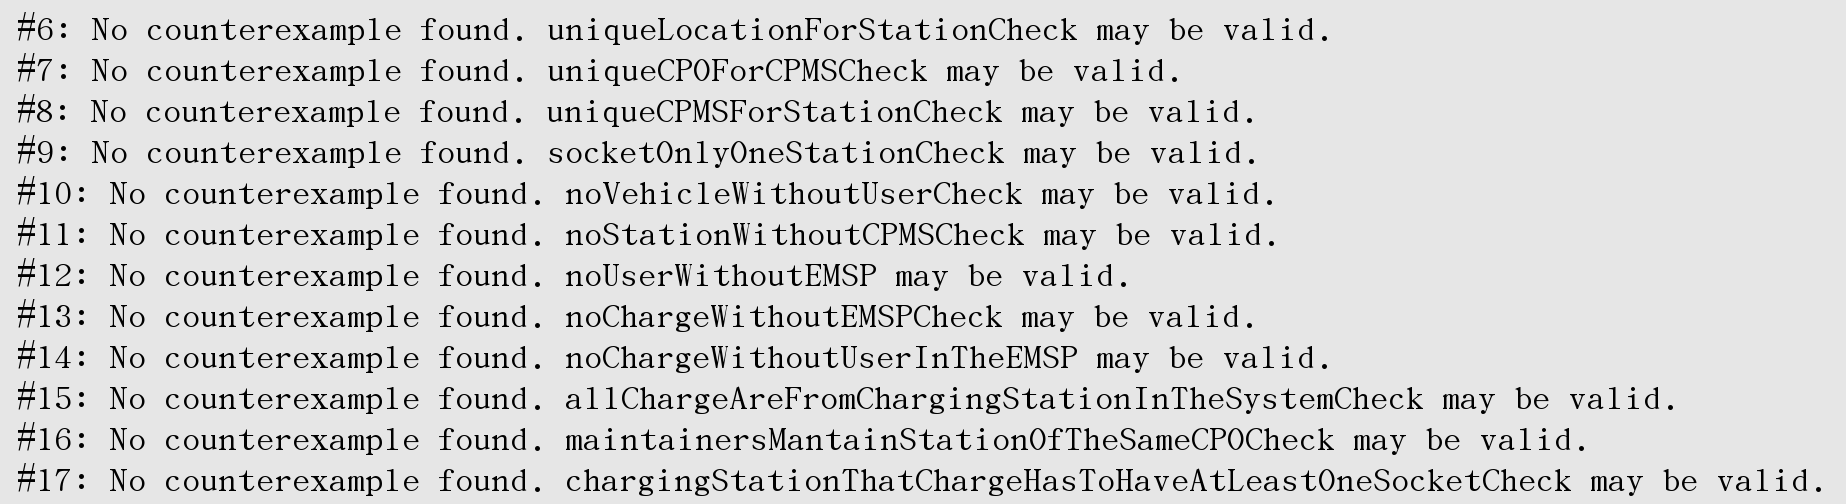
\includegraphics[keepaspectratio, width=16cm]{Alloy/AssertResult.png}
    \caption{Assertion output}
\end{figure}
\subsection{Word Generation}
Here is the code of the word generation.
\begin{verbatim}
    pred show() {
        #EMSP = 1
        #CPO>2
        #Charge>2
        #Vehicle>2
        #DefaultUser>2
    }
    run show
\end{verbatim}
And the generated word.
\begin{figure}[H]
    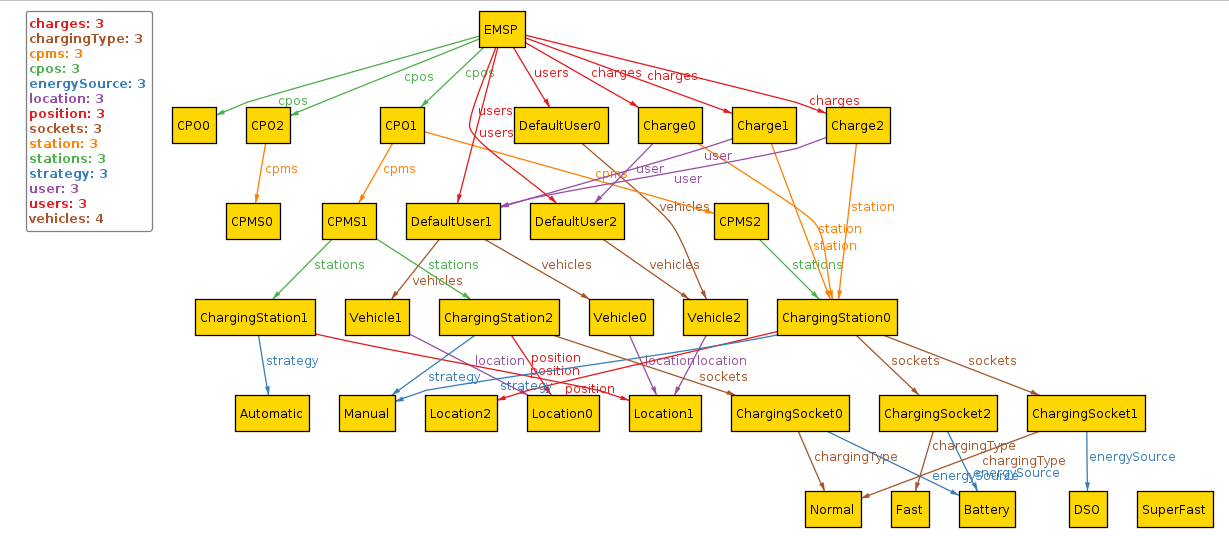
\includegraphics[keepaspectratio, width=16cm]{Alloy/WordGenerated.png}
    \caption{Generated Word}
\end{figure}
\clearpage